\documentclass[]{sig-alternate-10pt}
\usepackage{lmodern}
\usepackage{amssymb,amsmath}
\usepackage{ifxetex,ifluatex}
\usepackage{fixltx2e} % provides \textsubscript
\ifnum 0\ifxetex 1\fi\ifluatex 1\fi=0 % if pdftex
  \usepackage[T1]{fontenc}
  \usepackage[utf8]{inputenc}
\else % if luatex or xelatex
  \ifxetex
    \usepackage{mathspec}
  \else
    \usepackage{fontspec}
  \fi
  \defaultfontfeatures{Ligatures=TeX,Scale=MatchLowercase}
  \newcommand{\euro}{€}
\fi
% use upquote if available, for straight quotes in verbatim environments
\IfFileExists{upquote.sty}{\usepackage{upquote}}{}
% use microtype if available
\IfFileExists{microtype.sty}{%
\usepackage{microtype}
\UseMicrotypeSet[protrusion]{basicmath} % disable protrusion for tt fonts
}{}
\usepackage{hyperref}
\PassOptionsToPackage{usenames,dvipsnames}{color} % color is loaded by hyperref
\hypersetup{unicode=true,
            pdftitle={Analyzing the video delivery strategies of video providers},
            colorlinks=true,
            linkcolor=blue,
            citecolor=blue,
            anchorcolor=blue,
            urlcolor=blue,
            breaklinks=true}
\urlstyle{same}  % don't use monospace font for urls
\usepackage[backend=bibtex,style=numeric,hyperref=true,backref=true,maxnames=99]{biblatex}
\addbibresource{mybib.bib}
\usepackage{graphicx,grffile}
\makeatletter
\def\maxwidth{\ifdim\Gin@nat@width>\linewidth\linewidth\else\Gin@nat@width\fi}
\def\maxheight{\ifdim\Gin@nat@height>\textheight\textheight\else\Gin@nat@height\fi}
\makeatother
% Scale images if necessary, so that they will not overflow the page
% margins by default, and it is still possible to overwrite the defaults
% using explicit options in \includegraphics[width, height, ...]{}
\setkeys{Gin}{width=\maxwidth,height=\maxheight,keepaspectratio}
\setlength{\emergencystretch}{3em}  % prevent overfull lines
\providecommand{\tightlist}{%
  \setlength{\itemsep}{0pt}\setlength{\parskip}{0pt}}
\setcounter{secnumdepth}{5}

%\usepackage{caption}
%\renewcommand{\captionfont}{\small} %small fonts for caption
%\renewcommand{\captionlabelfont}{\small}

% \usepackage{url}
% \usepackage{balance}

%% Adding URL breaks
% \makeatletter
% \g@addto@macro{\UrlBreaks}{\UrlOrds}
% \makeatother

% \usepackage{lastpage}

%\usepackage[aboveskip=2pt]{subcaption} %for subfigures

%\setlength{\textfloatsep}{0pt} %spacing between figures and texts
%\setlength{\floatsep}{0pt} 
%\setlength{\dblfloatsep}{0pt}
%\setlength{\dbltextfloatsep}{0pt}
%\setlength{\abovecaptionskip}{0pt}
%\renewcommand{\footnotesize}{\scriptsize}

%\usepackage{etoolbox} % spacing between formula and text
%\apptocmd\normalsize{%
%\abovedisplayskip=0pt
%\abovedisplayshortskip=0pt
%\belowdisplayskip=0pt
%\belowdisplayshortskip=0pt
%}{}{}

%\let\oldfootnote\footnote %small footnote
%\renewcommand{\footnote}[1]{{\oldfootnote{\scriptsize #1}}}

\usepackage{graphicx}
\usepackage{multirow}
\usepackage{url}
\usepackage{xspace}
\usepackage{tabularx,ragged2e,booktabs,caption}
\usepackage{paralist}
\usepackage[american]{babel}
\usepackage[shortlabels]{enumitem}
\usepackage{amsmath,amssymb,times,graphicx,amsfonts}
\usepackage{courier,color,sped,url,wrapfig}
\usepackage{xspace}
\usepackage{balance}
\usepackage{enumitem}
\usepackage{epstopdf}
\usepackage{multirow}
\usepackage{booktabs}
\usepackage{url}
\usepackage{amssymb}
\usepackage{pifont}
\usepackage{subfigure}
\usepackage{tikz}
\usepackage{comment}
\usepackage{mathtools}
\usepackage{lastpage}
\usepackage{listings}
\usepackage{fancyvrb}

%\usepackage{fontspec}
%\setmainfont{Hoefler Text}
%\usepackage[noend]{algpseudocode}
%\usepackage{algorithmicx}
%\usepackage{algorithm}
\usepackage[]{algorithm2e}

%\usepackage[backref=page]{hyperref}

\newcommand{\cmark}{\ding{51}}%
\newcommand{\xmark}{\ding{55}}%


%%% Hotnets recommendation
% \setlength\paperheight {11in}
% \setlength\paperwidth {8.5in}
% \setlength{\textwidth}{7in}
% \setlength{\textheight}{9.25in}
% \setlength{\oddsidemargin}{-.25in}
% \setlength{\evensidemargin}{-.25in}

%%%%% Squeezing space before sections, subsections, and re-defining
%%%%% paragraphs
\makeatletter
\let\origsection\section
\let\origsubsection\subsection
\let\origparagraph\paragraph

\setlength{\textfloatsep}{5pt} %spacing between figures and texts
\setlength{\floatsep}{0pt} 
\setlength{\dblfloatsep}{0pt}
\setlength{\dbltextfloatsep}{0pt}
\setlength{\abovecaptionskip}{0pt}
\renewcommand{\footnotesize}{\scriptsize}

%\usepackage{etoolbox} % spacing between formula and text
%\apptocmd\normalsize{%
%\abovedisplayskip=0pt
%\abovedisplayshortskip=0pt
%\belowdisplayskip=0pt
%\belowdisplayshortskip=0pt
%}{}{}

%\let\oldfootnote\footnote %small footnote
%\renewcommand{\footnote}[1]{{\oldfootnote{\scriptsize #1}}}

\renewcommand\section{\@ifstar{\starsection}{\nostarsection}}
\renewcommand\subsection{\@ifstar{\starsubsection}{\nostarsubsection}}
\renewcommand\paragraph{\@ifstar{\starpara}{\nostarpara}}

%% Change these
\newcommand\sectionprelude{\vspace{1pt}}
\newcommand\sectionpostlude{\vspace{1pt}}
\newcommand\subsectionprelude{\vspace{1pt}}
\newcommand\subsectionpostlude{\vspace{1pt}}
\newcommand\paraspace{\vspace*{-1ex}}

\newcommand\nostarsection[1]{\sectionprelude\origsection{#1}\sectionpostlude}
\newcommand\starsection[1]{\sectionprelude\origsection*{#1}\sectionpostlude}

\newcommand\nostarsubsection[1]{\subsectionprelude\origsubsection{#1}\subsectionpostlude}
\newcommand\starssubection[1]{\subsectionprelude\origsubsection*{#1}\subsectionpostlude}

\newcommand\starpara[1]{\paraspace\noindent\origparagraph*{\textbf{#1}}}
\newcommand\nostarpara[1]{\paraspace\noindent\origparagraph*{\textbf{#1}}}

\providecommand\subparagraph[1]{\paraspace\noindent\origparagraph*{\textit{#1}}}

\makeatother

%%%% Backref magic
\DefineBibliographyStrings{english}{%
 backrefpage = {Cited on page},
 backrefpages = {Cited on pages},
}
\renewbibmacro{pageref}{%
 \iflistundef{pageref}
   {\printtext[parens]{Not Cited}} 
   {%
    \printtext[parens]{\ifnumgreater{\value{pageref}}{1}   
      {\bibstring{backrefpages}} 
      {\bibstring{backrefpage}}
      \printlist [pageref][-\value{listtotal}]{pageref}}}}    

\DeclareListFormat{pageref}{%
    % == 2 references
   \ifthenelse{\value{liststop} < 3}{\ifthenelse{\value{listcount}<\value{liststop}}{\hyperpage{#1} and }{\hyperpage{#1}}} %
   { % > 2 references
       \ifthenelse{\value{listcount}<\value{liststop}}
         {\hyperpage{#1}\addcomma\addspace}
         {\ifnumequal{\value{listcount}}{\value{liststop}}
           {and \hyperpage{#1}}
           {}%
         }%
   }%  
}


%\newcommand{\parab}[1]{\vspace*{0.5ex}\noindent\textbf{#1}}
\newcommand{\parae}[1]{\vspace*{0.5ex}\noindent\emph{#1}}

\newcommand{\ie}{i.e.,\xspace}


\title{Analyzing the video delivery strategies of video providers}
\author{
            \parbox{\textwidth}{\centering Georgios Papadimitriou, Zahaib Akhtar(Mentor)\\CSCI-651 Advanced Computer Communications \\[1ex]}
        }
\date{}

\begin{document}
\maketitle

\hypertarget{introduction}{%
\section{Introduction}\label{introduction}}

Video providers such as YouTube and Netflix are well understood today.
This is because of the attention they have received due to a large user
base. A number of research studies have explored their various aspects
including network architecture, user engagement and video delivery
mechanism etc. However, Internet video ecosystem consists of a large
number of small scale video providers which haven't received much
attention. While the bulk of the video traffic today is formed by big
providers, these small scale providers can be considered the tail of the
video traffic. The end goal of this project is to analyze the video
delivery strategies of these smaller providers and compare and contrast
them with popular providers.

\hypertarget{importance}{%
\paragraph{Importance}\label{importance}}

This project is interesting to the field, because it can provide insight
to the technologies used for video content delivery by small providers,
where video plays a supporting role in their businesses, such as news
outlets or online learning platforms. Additionally by analyzing and
comparing these data with what major providers are doing, such as
YouTube or Netflix, we can provide suggestions that will benefit the
smaller ones. Finally, from this project I will get a good understanding
of how the video content delivery pipeline works, and familiarize myself
with data analysis tools.

\hypertarget{challenges}{%
\paragraph{Challenges}\label{challenges}}

First, video delivery technologies differ between providers, because
they are trying to match them to their own needs and delivery
strategies. Due to this, we need to discover and specify a common way of
retrieving metadata, relevant to the delivered content, so we can
automate the acquisition process. Second, in order to provide useful and
reliable insights to the video delivery strategies we need to acquire
data for multiple videos and from as many video providers as possible.
This identifies the scale of the suggested analysis, and could be the
most challenging part of this project.

\iffalse

\hypertarget{mentor-meetings-log}{%
\section{Mentor Meetings Log}\label{mentor-meetings-log}}

\begin{itemize}
\item Meeting 1: General discussion about video streaming techniques and ways to get video URLs
\item Meeting 2: Discussion about how to select the set of video providers and which publisher categories we should focus on.
\item Meeting 3: Issue with Google search api, due to limitation on search domains and number of queries. Googler (https://github.com/jarun/googler) was proposed as a solution.
\item Meeting 4: Discussion about the specific streaming techniques we are going target in this study. Among the 4 popular techniques HLS, MPEG-DASH, HDS, Smooth Streaming we are going to focus on: 
\end{itemize}
\fi

\hypertarget{background}{%
\section{Background}\label{background}}

In order to serve video, providers typically use a \emph{Streaming
Protocol}. There are atleast four well known streaming protocols which
differ in popularity. These include 1. HTTP Live Streaming (HLS)
\autocite{hls} from Apple, 2. MPEG-DASH which is the Industry standard
protocol developed by the Motion Picture Experts Group (MPEG)
\autocite{dash}, 3. HTTP Dynamic Streaming Protocol (HDS) \autocite{hds}
implemented by Adobe and 4. The Smooth Streaming Protocol \autocite{mss}
which is implemented by Microsoft.

These streaming protocols specify a number of different characteristics
which are vital to video delivery. These include the network
encapsulation format for the video chunks, the set of available
bitrates, the duration of an individual chunk and the URL to fetch the
video content from. These are specified in what is called a
\emph{Manifest file}. Before a video player start playback, it downloads
the manifest file which informs the player about these attributes hence
enabling it to request video content and intelligently adapt bitrates
based on the network throughput.

Video providers use a number of different strategies to serve video
content. Their strategies can vary along a number of dimensions
including the choice of streaming protocol, the number of available
bitrate levels for adaptation, chunk duration and the content
distribution network (CDN). Their diversity along these dimensions can
be understood by analyzing the manifest files. We next describe our
methodology for selecting a candidate set of providers and obtaining
video manifest files for their video content.

\hypertarget{method}{%
\section{Methodology}\label{method}}

To bootstrap our measurement study we first need a list of content
providers that serve video. Second, we need a way to crawl through these
selected providers' websites to access the manifest files associated
with their video content.

\hypertarget{selecting-video-providers-to-study}{%
\subsection{Selecting Video providers to
study}\label{selecting-video-providers-to-study}}

We collect a set of video providers of interest by going through Alexa
top 500 website list \autocite{alexa}. Alexa provides a ranking of
websites based on the traffic, it also provides a ranking of websites
based on the type of content they serve. To pick popular video providers
we select websites from the ``Sports'' and ``News'' category. These
categories are important because most websites in this category
primarily serve video content. We pick a total of 15 websites.

\hypertarget{automated-crawling-and-data-collection}{%
\subsection{Automated crawling and data
collection}\label{automated-crawling-and-data-collection}}

We use and extend a number of open source tools to build a pipeline that
enables automated collection of the video manifest files. The following
steps constitute the pipeline. First, we extend an open source tool
called Googler \autocite{Googler} to harvest web links that contain
video content. Second, we use the harvested links to drive a Google
Chrome browser that loads the link and outputs the network requests
while it completes the page download. We do this by using the
chrome-remote-interface \autocite{ChromeRemoteInterface} which allows us
to remotely interact with a Google Chrome instance. Third, we filter and
collect the manifest URLs from the network log captured by Chrome.
Finally, we use custom scripts to download and process the manifest
files (and any sub-manifest files referenced in the main manifest file)
to record data of interest along the dimensions described above. We now
describe each of these steps in more detail and concretely define our
extensions to the different open source tools we use.

\hypertarget{googler}{%
\paragraph{Googler}\label{googler}}

Googler \autocite{Googler} is a tool written in Python that enables us
to perform google searches with custom queries. Googler has support for
regular google searches and searches targeting the ``News'' tab of the
results. Additionally it can navigate over the search results (with a
starting point and a total count of urls) and return them in either
plain text or json format. For our needs we have extended Googler to
perform searches targeting the ``Videos'' tab of the results. This way
we can narrow down the returned urls to the ones that contain videos in
them. An example of how we are using Googler in this project is the
following:

\begin{center}
\scriptsize
googler --noprompt --nocolor --json -V --start 10 --count 10 -w www.cnn.com ""
\end{center}

\hypertarget{chrome-remote-interface}{%
\paragraph{Chrome-Remote-Interface}\label{chrome-remote-interface}}

Chrome-Remote-Interface \autocite{ChromeRemoteInterface} is an interface
for the Chrome Debugging Protocol that helps instrument Google Chrome
and access its monitoring tools, such as console or networking, via
Javascript code. For our needs we are utilizing this tool to interact
with a Chrome browser instance, access the web pages that contain video
and log the network requests while the page loads. Since we are mainly
interested in obtaining the manifest files we do not need to wait for
the video to finish. The manifest file is downloaded before the video
starts to play. So we set a timeout of 30 seconds, a long enough value
for the manifest file to download. After the 30 seconds we terminate the
browser to free memory and continue the manifest file retrieval for the
next video.

\hypertarget{chrome}{%
\paragraph{Chrome}\label{chrome}}

Chrome is a web browser developed by Google. We are using Google Chrome
v.65 as a standard way of accessing urls containing video, in order to
hide our crawler behind a common web browser, interpret javascript at
runtime (sometimes it's required for the playback) and start the video
playback automatically. Also on the instance we are running we have
installed the AdBlock extension v.3.27.0, which is really useful in
avoiding advertisements where possible.

\hypertarget{custom-crawler}{%
\paragraph{Custom Crawler}\label{custom-crawler}}

Our crawler is responsible for combining all these individual components
into a single pipeline. It takes as input a text file that contains the
websites to be searched for pages that contain video, along with
starting points for the search and the total number of urls that are
going to be accessed. Currently the steps that the crawler takes to
retrieve the manifest files are the following:

\begin{enumerate}
\item Retrieve X number of urls for each website in the input file
\item Startup a Google Chrome instance in remote debug mode
\item For each url collected, interact with Google Chrome using chrome-remote-interface, access the url and retrieve the network requests
\item After the timeout period (currently 30 seconds) search the network requests for video manifest files based on known extensions (".m3u8", ".mpd", ".f4m")
\item Retrieve and store the contents of the manifest files with a simple HTTP GET
\end{enumerate}

It's important to state that we have implemented a simple logging and
checkpointing logic. From our crawler's execution we log the urls
fetched with googler, the accessed urls with their generated network
requests, and Google Chrome's debug output. With this approach we can
request to get more urls and access them without starting over by simply
increasing the number of urls we want to access. This can be achieved
because the crawler is aware of the working directory and checks the
logs and created files before performing an action.

\begin{figure*}
\centering
\fbox{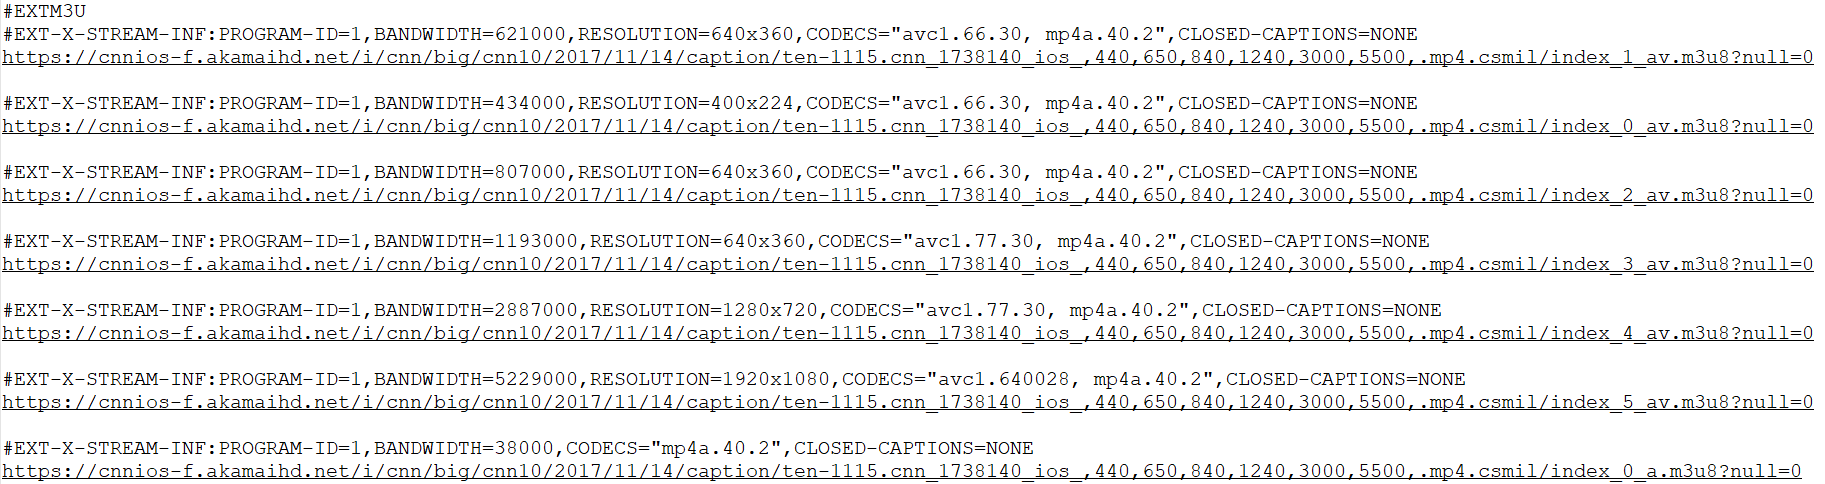
\includegraphics[width=0.9\textwidth]{m3u8_example.png}}
\caption{Master Manifest File Example}
\end{figure*}
\begin{figure*}
\centering
\fbox{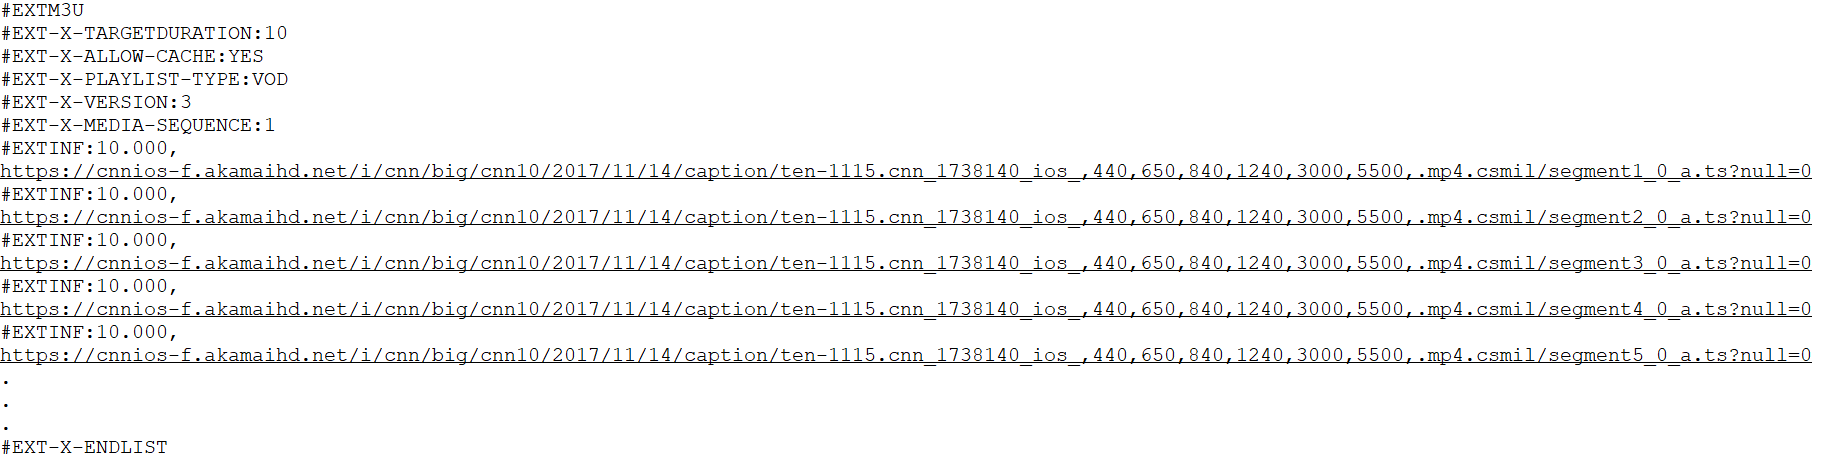
\includegraphics[width=0.9\textwidth]{m3u8_sub_example.png}}
\caption{Sub Manifest File Example}
\end{figure*}

\hypertarget{example-manifest-file}{%
\section{Example Manifest File}\label{example-manifest-file}}

Figure 1 presents an example of an HLS master manifest file collected
from a video delivered by CNN.COM, and Figure 2 presents a portion from
one of its sub-manifest files. The master and the sub manifest files
contain a wealth of information describing the publisher's video
delivery strategy for the given video. By parsing and analyzing its
content we can derive information such as:

\begin{itemize}
\item The CDN that hosts the manifest files. In this case the CDN is Akamai, as evident by the fully qualified domain name (\texttt{https://cnnios-f.akamaihd.net}) in the URL. If the URL doesn't directly provide information about the origin we can perform a \texttt{whois} lookup to determine the owner the domain.
\item The number of alternative video bitrates offered for the specific video, by counting the unique index files. In this case seven different bitrates are offered.
\item The exact bitrate levels (\texttt{BANDWIDTH} tag), codecs and video resolution used for each alternative stream, by interpreting the "preamble" of each index file.
\end{itemize}

On the other hand the sub-manifest file contains the actual chunks
streamed to the device for the video playback. From this file we can get
information about:

\begin{itemize}
\item The CDN that hosts the actual chunks of the video streamed
\item The type of video that is being viewed. In this case the video is pre-recorded on demand video (VOD) as given by the \texttt{EXT-X-PLAYLIST-TYPE} tag. Alternatively it could have been a live stream.
\item The time segment of the video each chunk covers, by parsing the preamble of the file. Specifically the \texttt{EXT-X-TARGETDURATION} tag provides us information about the duration of the chunk. In this case the chunk duration is 10 seconds.
\end{itemize}

\begin{table}
\centering
\resizebox{0.85\columnwidth}{!}{%
 
\begin{tabular}{|l|l|l|}
\hline
\textbf{Publisher}     & \textbf{Category} & \textbf{Alexa Rank} \\ \hline\hline
www.cnn.com                   & News              &            2         \\ \hline
www.nytimes.com             & News              &            3         \\ \hline
www.bbc.com                    & News              &           6          \\ \hline
www.foxnews.com            & News              &           10         \\ \hline
www.weather.com             & News              &           11         \\ \hline
www.huffingtonpost.com   & News              &           14         \\ \hline
www.usatoday.com           & News              &           16          \\ \hline
www.bloomberg.com         & News              &          17          \\ \hline
www.cnbc.com                   & News              &          19          \\ \hline
www.wsj.com                      & News              &          20         \\ \hline
www.espn.com                   & Sports            &           1            \\ \hline
www.nba.com                     & Sports            &           7            \\ \hline
www.premierleague.com    & Sports            &           14          \\ \hline
www.wwe.com                    & Sports            &           31          \\ \hline
\end{tabular}%
 
}
\caption{The providers we study, their Alexa categories and rank within the category}
\label{table:pub_table}
\end{table}

\hypertarget{analysis-and-results}{%
\section{Analysis and Results}\label{analysis-and-results}}

Our analysis is performed on 15 different content providers. As
discussed in \S\ref{method} these providers were selected based on the
Alexa top websites ranking within different categories. Table
\ref{table:pub_table} shows the content providers, their categories and
the rank in their respective categories. In particular, of the 15
providers we study, 11 primarily serve News content and the remaining 4
serve Sports content. Further, notice that all the providers are
prominent in their categories as shown by their Alexa rank. \iffalse

\begin{itemize}
\item www.usatoday.com
\item www.cnbc.com
\item www.nytimes.com
\item www.premierleague.com
\item www.espn.com
\item www.wsj.com
\item www.bbc.com
\item www.foxnews.com
\item www.wwe.com
\item www.huffingtonpost.com
\item www.weather.com
\item www.bloomberg.com
\item www.cnn.com
\item www.nba.com
\item www.nbcolympics.com
\end{itemize}
\fi

\hypertarget{bitrate-values}{%
\subsection{Bitrate Values}\label{bitrate-values}}

Figure \ref{fig:bitrate1} presents the average number of different
bitrates offered per video by the providers. Almost all the provider
have on average more than 4 bitrates available for a specific video and
some of them offer over 8 different options. Additionally observing
Figure \ref{fig:bitrate2} we can tell the distribution of bitrates.

\begin{figure}
\centering
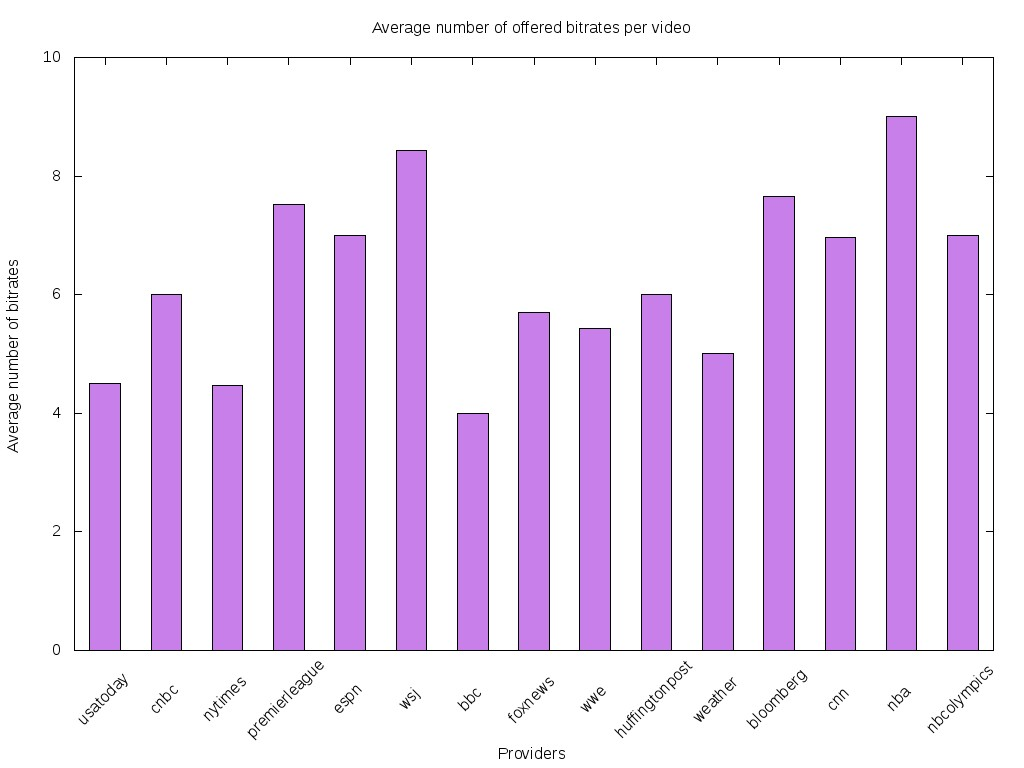
\includegraphics[width=0.4\textwidth]{bitrate_bar_plot.jpg}
\caption{Number of bitrate levels offered by providers}
\label{fig:bitrate1}
\end{figure}

\begin{figure}
\centering
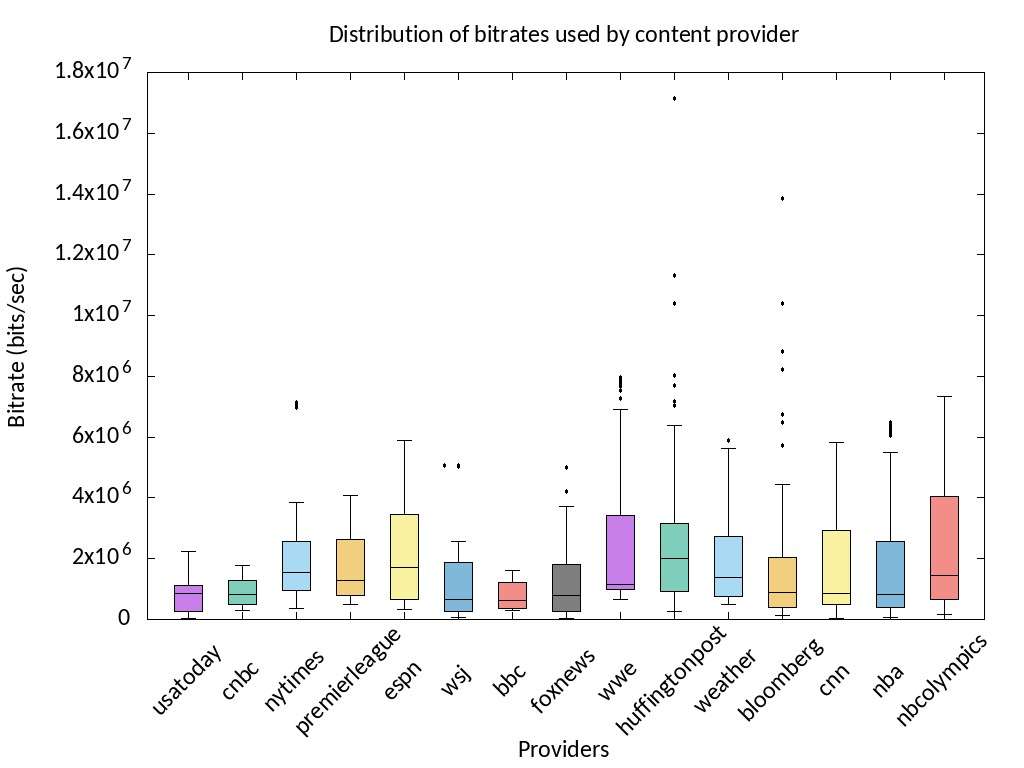
\includegraphics[width=0.4\textwidth]{bitrate_box_plot.jpg}
\caption{Levels of different bitrates offered by providers}
\label{fig:bitrate2}
\end{figure}

\hypertarget{cdns}{%
\subsection{CDNs}\label{cdns}}

In Figure \ref{fig:cdn1} we present the number of different CDNs used by
the providers, that we discovered. Most of the providers use at most one
CDN, but there are others opting for two or three. However, as we
observed, this was done for different sections of their video
categories. In Figure \ref{fig:cdn2} we show which CDNs we found to be
more by the providers. Akamai Technologies is used by 73\% of the
crawled providers, in second place there is Fastly that appeared in 20\%
of the providers, Limelight and Brightcove appeared in 13\% of the
providers and Amazon AWS in just under 7\%.

\begin{figure}
\centering
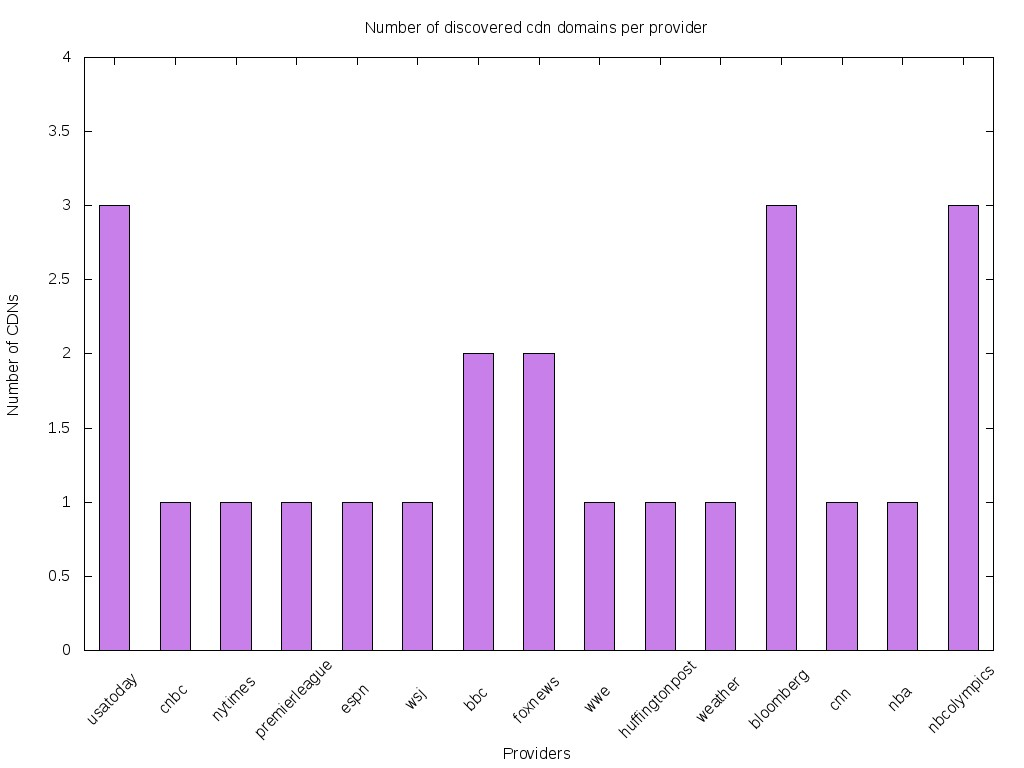
\includegraphics[width=0.4\textwidth]{cdn_bar_plot1.jpg}
\caption{Number of CDNs used by different publishers}
\label{fig:cdn1}
\end{figure}
\begin{figure}
\centering
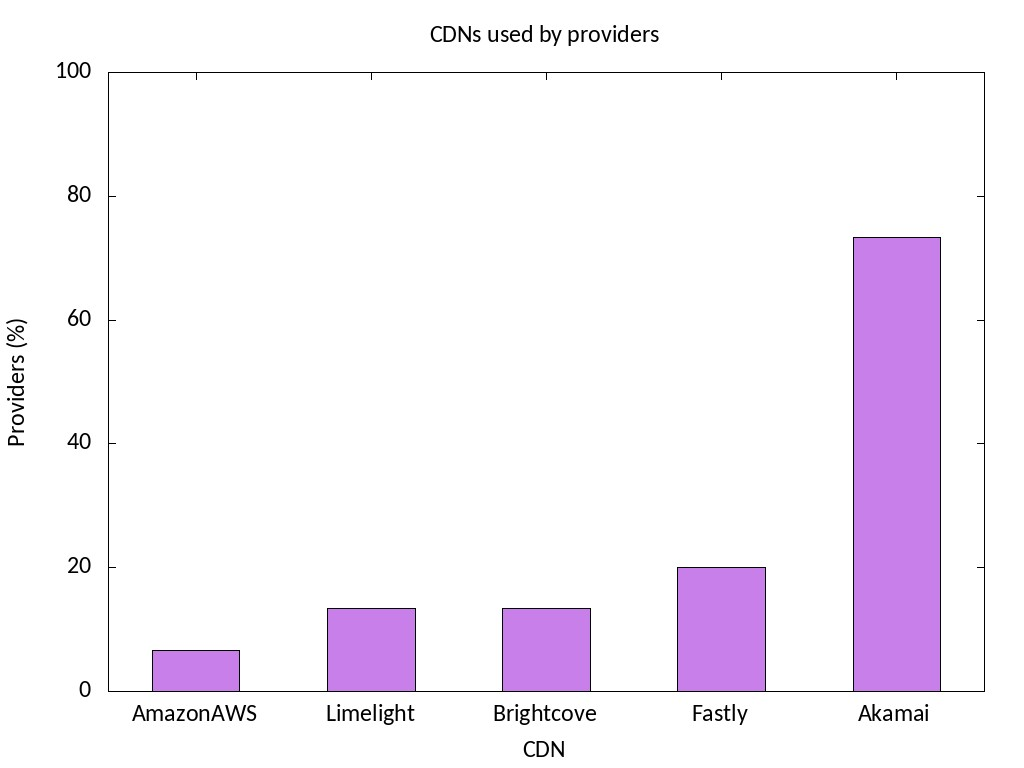
\includegraphics[width=0.4\textwidth]{cdn_bar_plot2.jpg}
\caption{Most popular CDNs among different providers}
\label{fig:cdn2}
\end{figure}

\hypertarget{chunk-target-duration}{%
\subsection{Chunk Target Duration}\label{chunk-target-duration}}

Chunk size can vary from video to video and from chunk to chunk.
However, each provider specifies a target chunk size that video chunks
tend to converge to. In Figure \ref{fig:chunk1} we present the number of
different video chunk sizes offered by each provider. The majority of
the providers is using one target chunk size, but there are some
providers offering multiple chunk target durations throughout their
videos, probably because of the video length. Also, by analyzing the
individual step of each chunk in videos, some of the providers offer
smaller chunks in the beginning of the video for faster playback start.
Figure \ref{fig:chunk2} presents how many providers are using a target
chunk duration. 46\% of the providers is using chunks of 10 seconds,
33\% uses chunks of 6 seconds, 20\% uses chunks of 4 and 7 seconds, 13\%
uses chunks of 11 seconds, and under 7\% uses chunks of 9 seconds and 12
seconds.

\begin{figure}
\centering
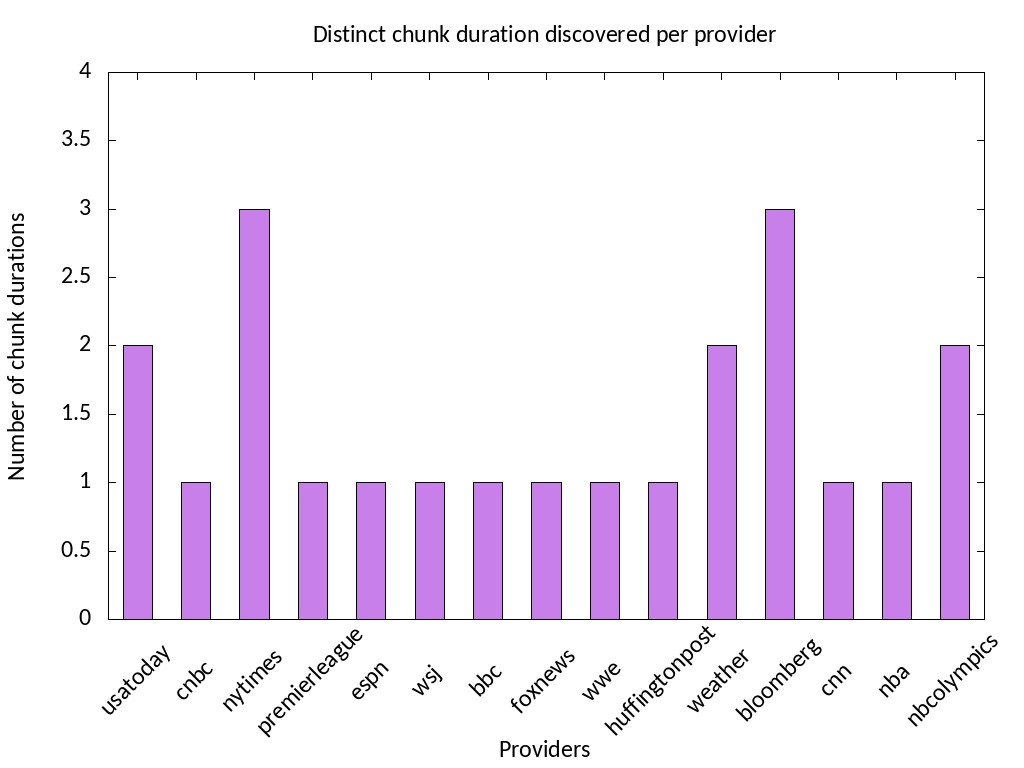
\includegraphics[width=0.4\textwidth]{chunk_targetduration_bar_plot1.jpg}
\caption{Number of different chunk durations used by different publishers}
\label{fig:chunk1}
\end{figure}
\begin{figure}
\centering
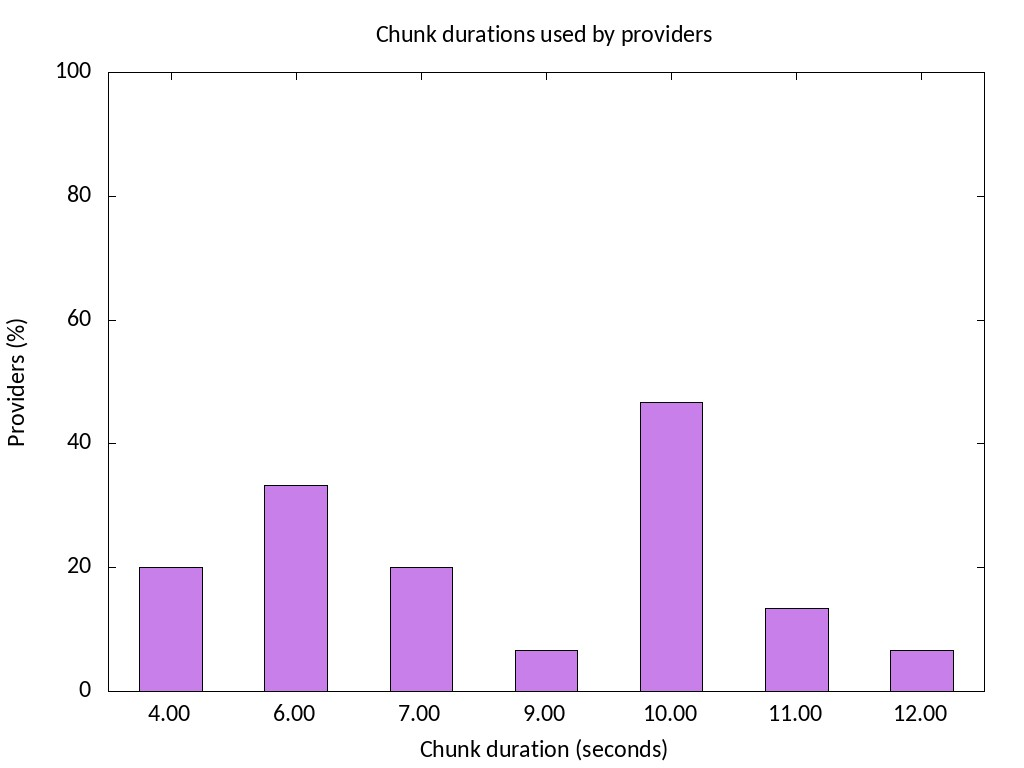
\includegraphics[width=0.4\textwidth]{chunk_targetduration_bar_plot2.jpg}
\caption{Popularity of different chunk duration used by publishers}
\label{fig:chunk2}
\end{figure}

\hypertarget{codecs}{%
\subsection{Codecs}\label{codecs}}

With Figure \ref{fig:codecs1} we present the number of different codecs
used by the providers. This graph brakes down the codecs to audio only
and video. There are 7 providers offering audio only streams, and
usually these were marked with captions as well. Most of the providers
offer their content in about 4 different codec configurations, and there
are two (Huffingtonpost and Bloomberg) where we discovered 13 different
codec configurations. Here we should note that for
``www.premierleague.com'' we haven't tracked codecs because they were
missing from the manifest files. In Figure \ref{fig:codecs2} we present
the codecs and their popularity among the providers. For video
``avc1.66.30, mp4a.40.2'' and ``avc1.77.30, mp4a.40.5'' were the most
popular, and for audio only ``mp4a.40.2''.

\begin{figure}
\centering
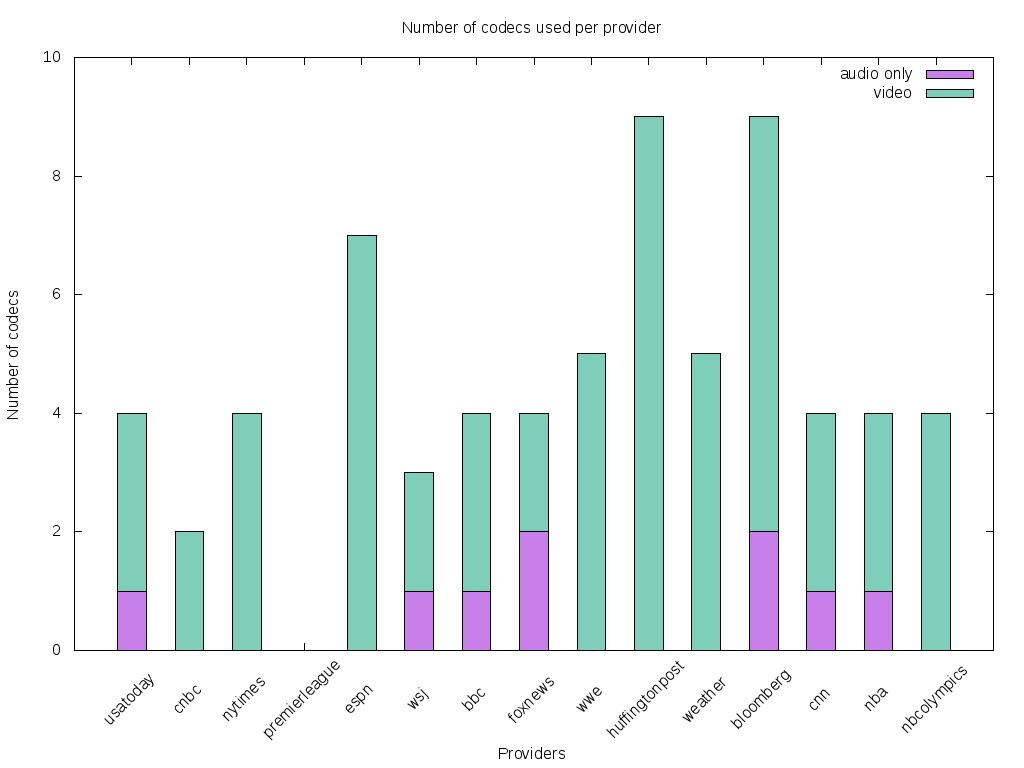
\includegraphics[width=0.4\textwidth]{codecs_bar_plot1.jpg}
\caption{Different number of codecs used by publishers}
\label{fig:codecs1}
\end{figure}
\begin{figure}
\centering
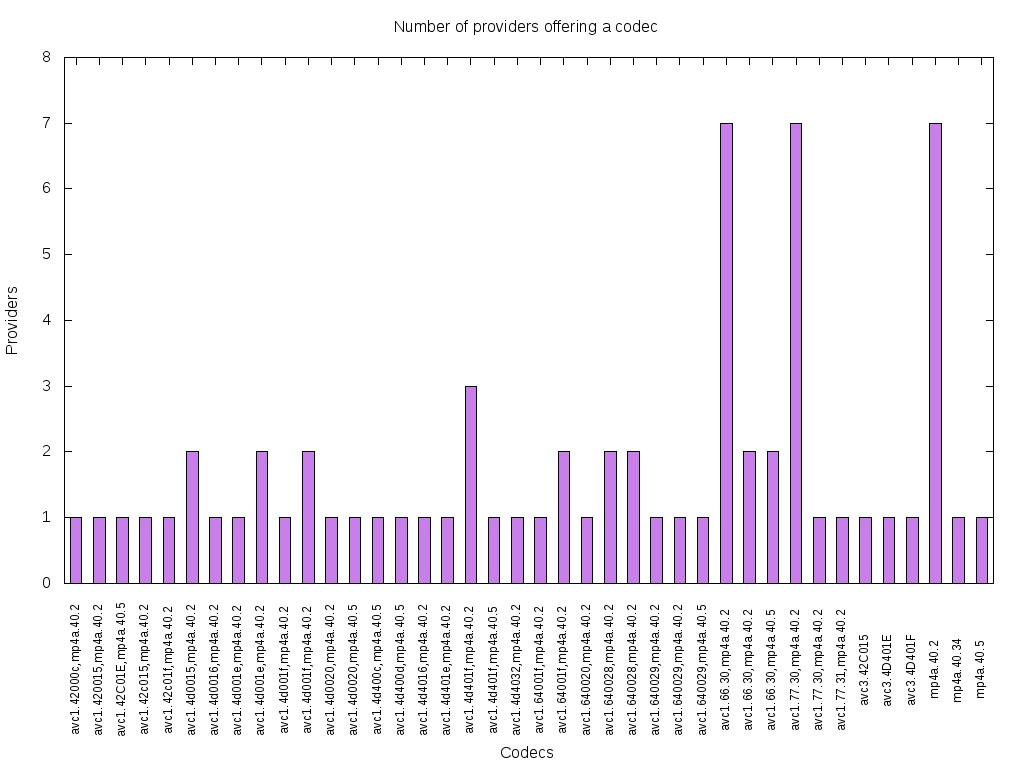
\includegraphics[width=0.4\textwidth]{codecs_bar_plot2.jpg}
\caption{Popularity of different codecs}
\label{fig:codecs2}
\end{figure}

\hypertarget{protocols}{%
\subsection{Protocols}\label{protocols}}

Figure \ref{fig:protocols} depicts the protocols used by the providers.
The most popular protocol used among them is HTTP Live Streaming (HLS).
Almost all the providers are using HLS, and the dominant version is
HLS.v3. BBC on the other hand is using MPEG-DASH for it's new videos and
for the old ones (before 2015) is still using Flash. We also considered
Fifa.com in this study, which is using Flash for all its videos, but we
don't have more date, because it was extremely difficult to study how
they transfer the video files. Note: \text\_it\{There were some of the
providers that didn't specify the HLS version in their manifest files,
and that's why there is one HLS entry with no version.\}

\begin{figure}


\centering
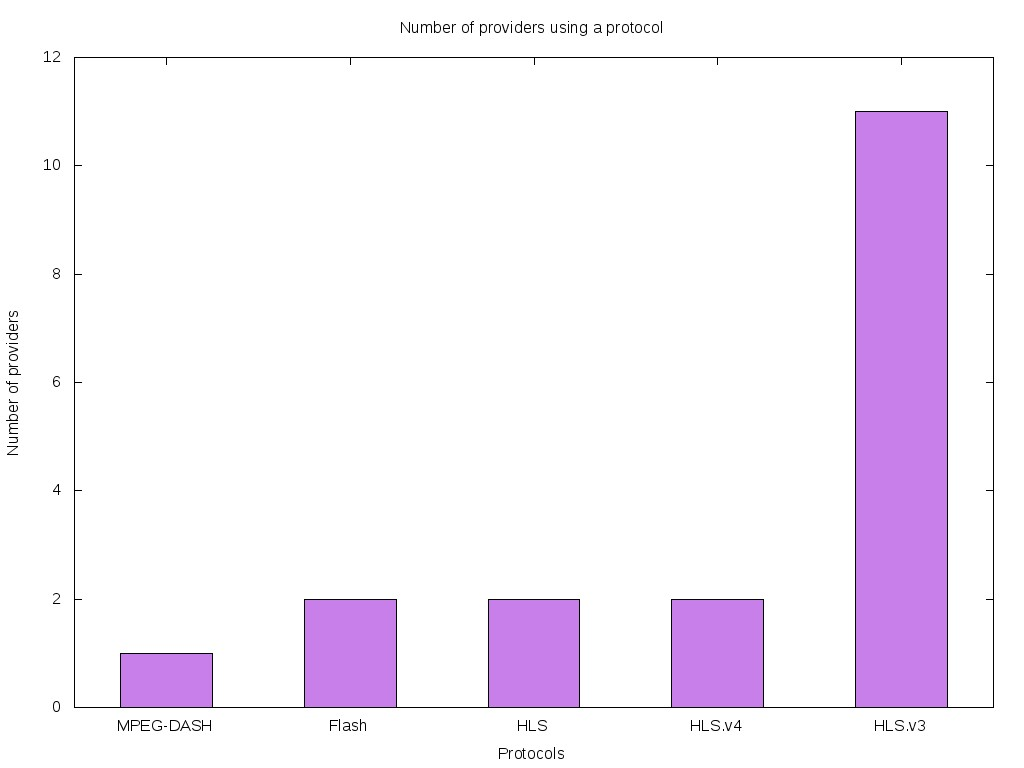
\includegraphics[width=0.4\textwidth]{protocol_bar_plot.jpg}
\caption{Popularity of different streaming protocols used by publishers}
\label{fig:protocols}
\end{figure}

\hypertarget{resolution}{%
\subsection{Resolution}\label{resolution}}

Along with different bitrates providers also give options for different
video resolutions in their manifest files. Figure \ref{fig:resolution1}
shows the average number of resolutions offered from each provider per
video. All providers give more than two resolution options and sport
sites, such as ``www.nba.com'' and ``www.nbcolympics.com'' offer more
than six. Observing Figure \ref{fig:resolution2}, we can tell that there
are providers offering different resolutions throughout their videos.
For example ``ww.usatoday.com'' offers twelve video resolutions
throughout their site but only 3 on average for each video. This is also
true for ``www.nytimes.com'' and ``www.huffingtonpost.com''. In Figure
\ref{fig:resolution3} we display the resolutions found in provider's
videos. Most popular resolutions are 640x360 and 1280x720 (720p), with
100\% of providers offering them. Next in popularity is 960x540 (old
iPhone), offered by more than 65\% of the providers, and 1920x1080
offered by more than 50\% of the providers.

\begin{figure}
\centering
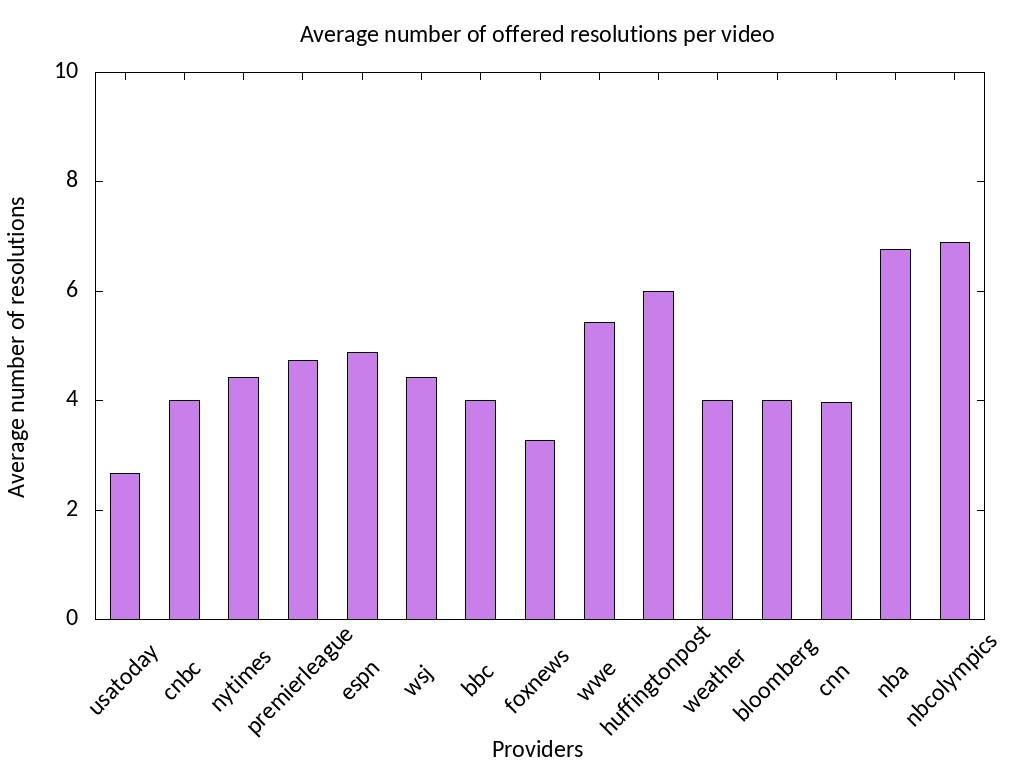
\includegraphics[width=0.4\textwidth]{resolution_bar_plot1.jpg}
\caption{Number of resolutions offered by different publishers}
\label{fig:resolution1}
\end{figure}
\begin{figure}
\centering
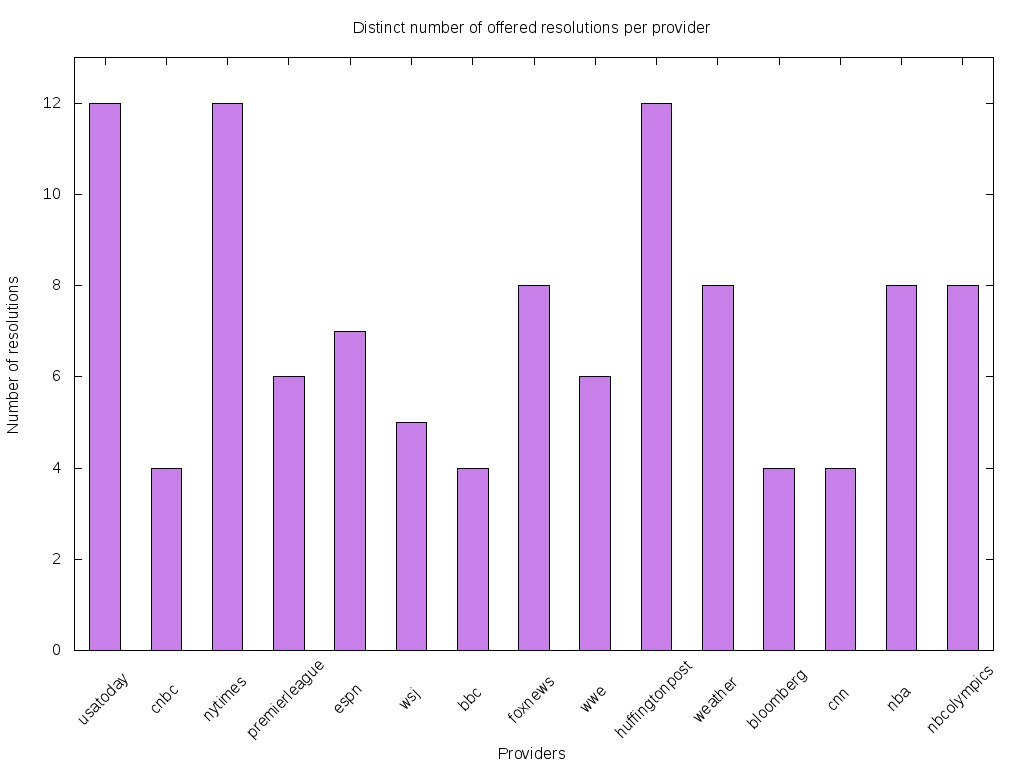
\includegraphics[width=0.4\textwidth]{resolution_bar_plot2.jpg}
\caption{Resolution 2}
\label{fig:resolution2}
\end{figure}
\begin{figure}
\centering
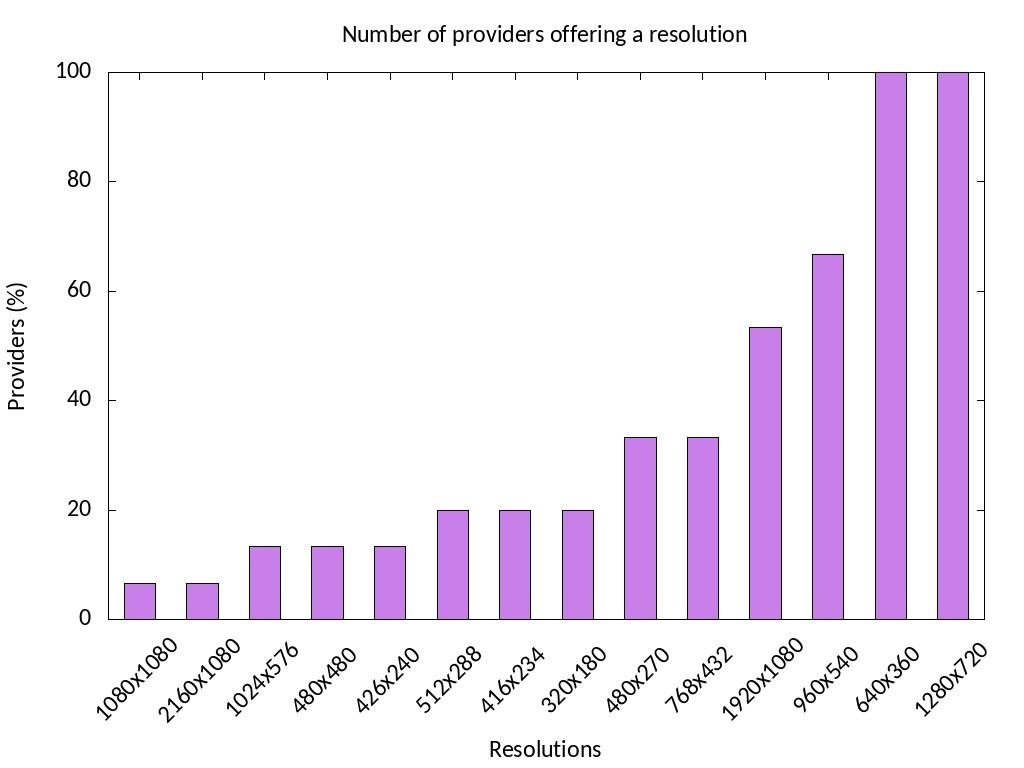
\includegraphics[width=0.4\textwidth]{resolution_bar_plot33.jpg}
\caption{Number of providers offering a resolution}
\label{fig:resolution3}
\end{figure}

\hypertarget{related-work}{%
\section{Related Work}\label{related-work}}

Due to their popularity, video serving systems have been the subject of
a large body of work. YouTube alone has been the subject of numerous
studies over the years.
\autocites{Adhikari10}{mattgoogle}{Gill07}{Zink09}{Cha07}{sanjay11}{Torres11}{upload}{prefixcounting}.
Together these works have studied a number of YouTube's aspect,
including the architecture and its evolution, serving strategy,
characterization of videos and the user access patterns etc. Netflix,
another major provider has also received much attention, where
researchers have characterized its delivery strategy in
\autocites{netflix}{BB}.

In addition to these well known systems, researchers have also focused
on a on-demand TV publisher \autocites{paytv}{ondemand}, as well as
novel video delivery systems which allow users to broadcast live streams
\autocites{ucsblive}{periscope}. The thread that unites these works is
their specific focus on one or a handful of online providers, in
contrast this project focuses on understanding the diversity at a macro
level across a large number of online video providers. One piece of work
that is somewhat closer to this project is \autocite{ottgorilla}. This
work analyzes video traffic generated from a large number of users of a
prominent cellular services provider. Their results show that in 2011,
HLS, a video streaming protocol contributed to one third of the total
video traffic.

\printbibliography[title=Bibliography]

\end{document}
